\documentclass[a4paper,12pt]{article}
\usepackage[hidelinks]{hyperref}
\usepackage{graphicx}
\usepackage{float}
\usepackage{caption}

%% Title Page 
\begin{document}
\title{\Huge Functional Requirements Document Specification \\ 
	 Project: \\ 
	Cafeteria Management System: Resolve}
\author{
         \underline{T-RISE}\\
          Rendani Dau (13381467) \\
	Elana Kuun (12029522) \\
	Semaka Malapane (13081129) \\
	Antonia Michael (13014171) \\
	Isabel Nel (13070305)\\ \\
	https://github.com/toniamichael94/MainProjectCOS301}

\date{\today}
 
%\documentclass[12pt]{article}


\maketitle
\break

%% Make table of contents
\tableofcontents
\break

\begin{tabu} to 0.8\textwidth { | X[l] | X[c] | X[r] | }
 \hline
\textbf{Document Title} & Functional Requirements Document \\
 \hline
 \textbf{Document Identification}  & Document 0.0.1  \\
\hline
 \textbf{Author}  & Rendani Dau, Isabel Nel, Elana Kuun, Semaka Malapane, Antonia Michael \\
\hline
\textbf{Version} & 0.0.1 \\
\hline
\textbf{Document Status} & First Version - contains two use cases \\
\hline
\end{tabu}



\begin{table}[h!]
\centering
 \begin{tabular}{||c c c c||} 
 \hline
 \textbf{Version} & \textbf{Date} & \textbf{Authors} & \textbf{Summary} \\ [0.5ex] 
 \hline\hline
 0.0.1 & 29 May 2015 &  Author  & Rendani Dau, Isabel Nel, Elana Kuun, Semaka Malapane, Antonia Michael  & First draft contains first two use cases \\ 
 2 & 7 & 78 & 5415 \\  [1ex] 
 \hline
 \end{tabular}
\end{table}

\pagebreak



%%now begin document

%%---------------------------------  INTRODUCTION -------------------------------------------
\section{Introduction}
This document contains the functional requirements specification, architecture requirements and testing for the Resolve Cafeteria Management System that will be created for Software Engineering (COS 301) at the University of Pretoria 2015, by the group T-RISE. In this document we will thoroughly discuss and layout the project's functional requirements to provide a clear view of the system as a whole. An agile approach is being followed, hence the main use cases that this document will be focussing on are placing orders and managing a user profile. These will be explored in quite some detail.  The agile method involves an interactive and incremential method of managing and designing the system. 
%% ------------------------------ VISION ------------------------------------------------------
\section{Vision}
The vision of this project is to implement a flexible, pluggable, fully functional software application that will be maintainable, with detailed supporting documentation and an instruction manual for the Cafeteria Management System. This system will assist in managing the cafeteria's inventory/stock, placing orders made by employees, generating bills, and sending the appropriate information to the right parties.  

%%---------------------------------- BACKGROUND -----------------------------------------
\section{Background}
As specified in the project proposal document from Resolve, the cafeteria is currently cash only and does not accept bank cards or electronic payments. This makes it inconvenient for employees as they have to have cash on hand if they want to purchase anything from the cafeteria. Employees might choose to buy somewhere else where they can use another form of payment. The employees have to use fuel and time, and this does not bring in the maximum amount of income to the cafeteria, hindering its growth and improvement.\\

Resolve is therefore looking for a means to accept payments from employees for the canteen using their employee access cards or access card numbers. The amount spent at the cafeteria can then be deducted from their salary at the end of the month.\\

After our first meeting with the client, they brought to our attention that at times the cafeteria does not have enough stock to provide some of the menu items, therefore the managing of inventory and stock will also be part of the system. The system will also predict what inventory/stock needs to be bought for the next week in order to avoid shortcomings. At the end of each month, the bill for that month will be sent to either payroll or to the employee. This option is configurable from the user's profile. The employee can also set a spending limit for each month. The system will also have a maximum limit that users cannot exceed.
 
%%--------------------------------------- FUNCTIONAL REQUIREMENTS--------------------------------
\section{Functional Requirements and Application Design}
In this section we will discuss the functional requirements. \\

%% ---------------USE CASES -------------------
\subsection{Use Cases }
Below is a list of all the use cases we have identified:

\begin{itemize}

\item Authentication
\item Register
\item Manage Profile
\item Place Order
\item Notify
\item Manage Inventory
\item Report

\end{itemize}


%% ---------------USE CASE PRIORITIZATION -------------------
\subsection{Use Case Prioritization}
Below the use cases mentioned above will be catagorized as critical, important or nice to have.

\begin{itemize}

\subsubsection{Critical}
\item Authentication \\
This is a critical use case due to the fact that you cannot send through any order if you are not logged in. In such a case you will only be able to view the menu. 
 
\item Register \\
This is a critical use case because you can not log into the system if you have not been registered on the system. Furthermore, if you are not logged in, you can not place orders.

\item Place Order\\
This is critical due to the fact that the main functionality of the system revolves around the ability to place orders at the cafeteria as well as other activities relating to that. 

\subsubsection{Important}
\item Manage Profile \\
This use case is considered important because the user must be able edit their profile by resetting their personal spending limits and changing their email and passwords. The user must also be able to view his/her account history and current bill. It is crucial that the user is able to configure spending limits according to their own preferences as well as keep track of monthly purchases.

\item Manage Inventory \\
This use case is considered important, because it deals with incrementing stock that has been added and decrementing stock when it is purchased or expired. It also deals with the cafeteria manager marking orders as completed.

\item Reporting \\ 
This use case is considered important because users must be able to print a billing report. They should also have the option of sending their montlhly bill to payroll where it will be deducted from their salaries. A history of all the orders that have taken place on the system can also be printed. 

\subsubsection{Nice to have}
\item Notify \\
This is classified as nice to have as it includes notifying a user when their order is ready for collection, as well as other notifications, such as notifying the cashier or cafeteria manager that they are low on certain inventory.  The system is not dependant on this functionality.

\end{itemize}

%%--------------- USE CASE/SERVICE CONTRACTS --------------
\section{Modular System}
The system will be built using a modular approach to allow more modules to be added at a later stage. This will also provide for pluggability and integratibility of the system.

\subsection{High level use case diagram of the CMS}
\begin{figure}[H]
  \centering
    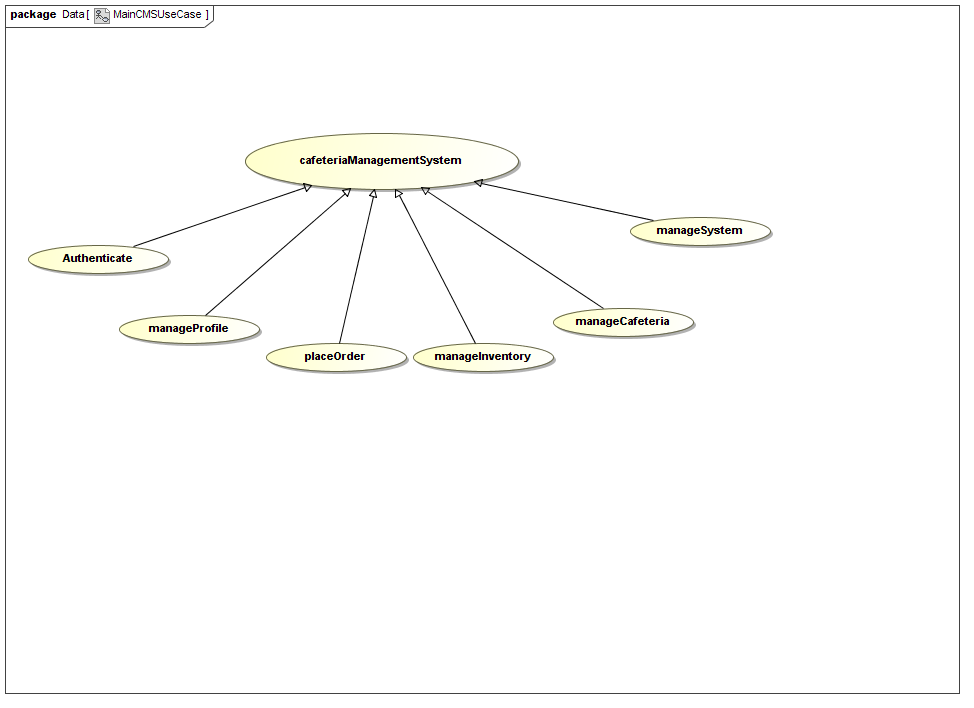
\includegraphics[width=1.0\textwidth]{images/CMSUseCase.png}
    \caption{Cafeteria Management System Use Case} 
\end{figure}
The core of the system is a cafeteria management system that will provide functionality such as allowing users to place orders once they have registered and logged on to the system. Different types of users will have different privileges. 

\subsection{Place Orders Module}
The main functionality the system serves to provide, is  to allow the user to use their access card number to purchase food items from the cafeteria via the system. This use case diagram indicates the functionality around placing orders, such as CheckProductAvailability and checkLimits, which are the use cases of this module.
\begin{figure}[H]
  \centering
    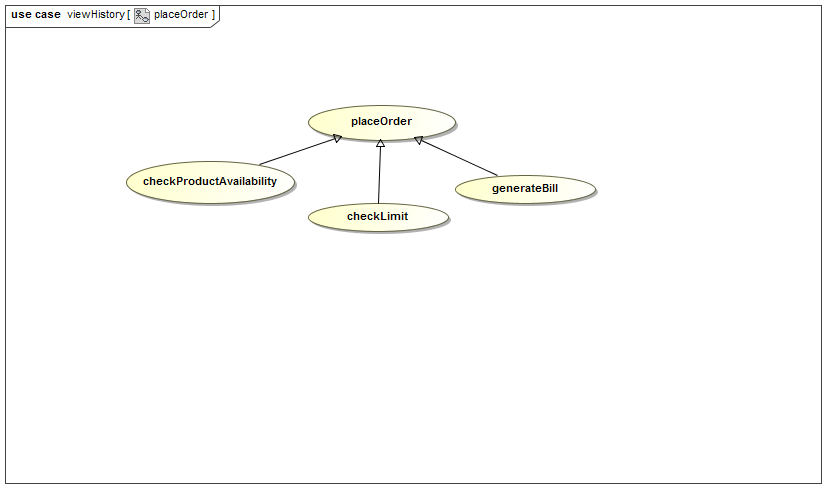
\includegraphics[width=1.0\textwidth]{images/placeOrder.png}
    \caption{The use case for placing an order} 
\end{figure}
 
\subsubsection{CheckProductAvailability}
The service contract and activity diagram for CheckProductAvailability follow. CheckProductAvailability falls under the use case for Place Orders (refer to page 7 - figure 2 to view this use case diagram). The system will check whether the product that the user has selected to purchase is currently in stock.
\begin{figure}[H]
  \centering
    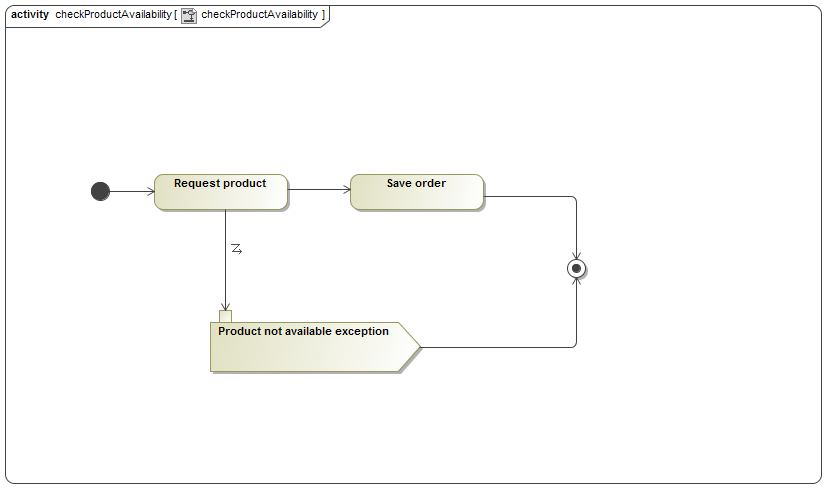
\includegraphics[width=1.0\textwidth]{images/checkProductAvailability.png}
    \caption{The activity diagram for checking product availibilty } 
\end{figure}
 
\begin{figure}[H]
	\centering
	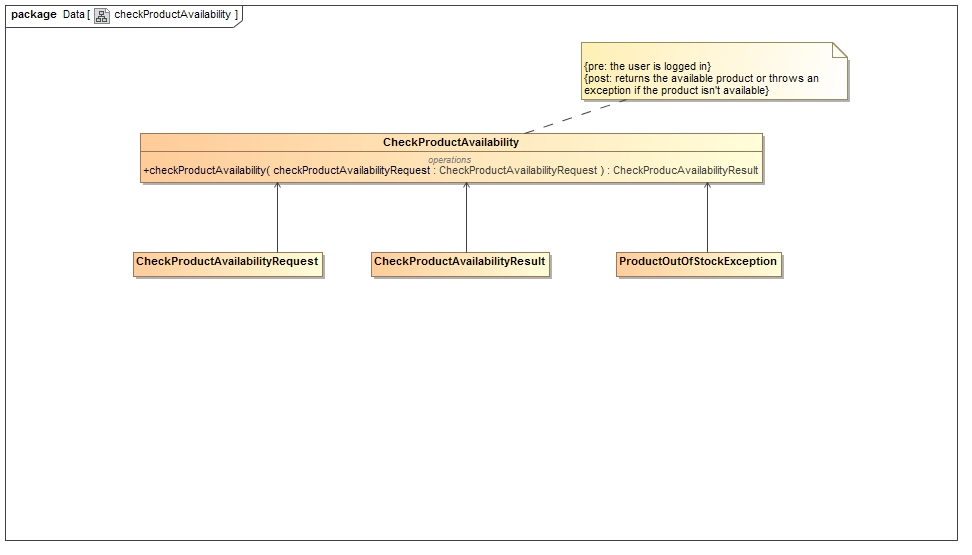
\includegraphics[width=1.0\textwidth]{images/checkProductAvailabilitySC.jpg}
	\caption{The service contract for checking product availabilty}
\end{figure}

\subsubsection{checkLimit}
The service contract and activity diagram for checkLimit follow. checkLimit falls under the use case for Place Orders (refer to page 7 to view this use case diagram). The system will be able to view the user's personal limit to make sure that the total of the bill is not larger than the users spending limit. 
\begin{figure}[H]
  \centering
    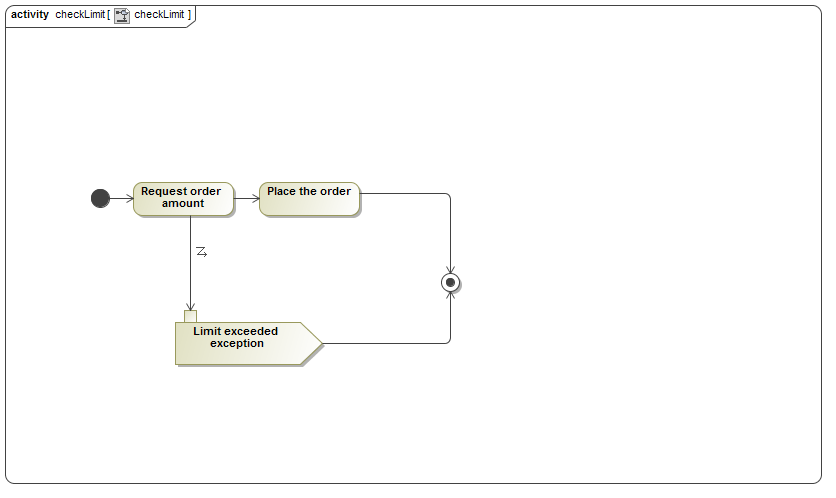
\includegraphics[width=1.0\textwidth]{images/checkLimit.png}
    \caption{The activity diagram for checking limits} 
\end{figure}

\begin{figure}[H]
	\centering
	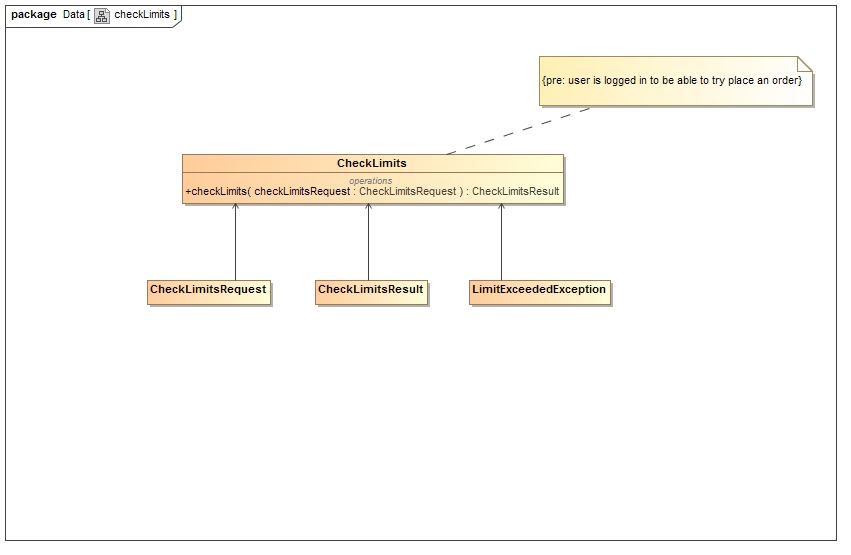
\includegraphics[width=1.0\textwidth]{images/checkLimitsSC.jpg}
	\caption{The service contract for checking limits}
\end{figure}

\subsection{Manage Profile Module}
 The user will be allowed to customize various settings such as resetting his/her personal limit, changing password and email, displaying the bill and viewing favourites. The following use case diagram indicates the above mentioned functionality around managing the profile. Hence, it has the use cases generateFavourite and edit profile.

\begin{figure}[H]
  \centering
    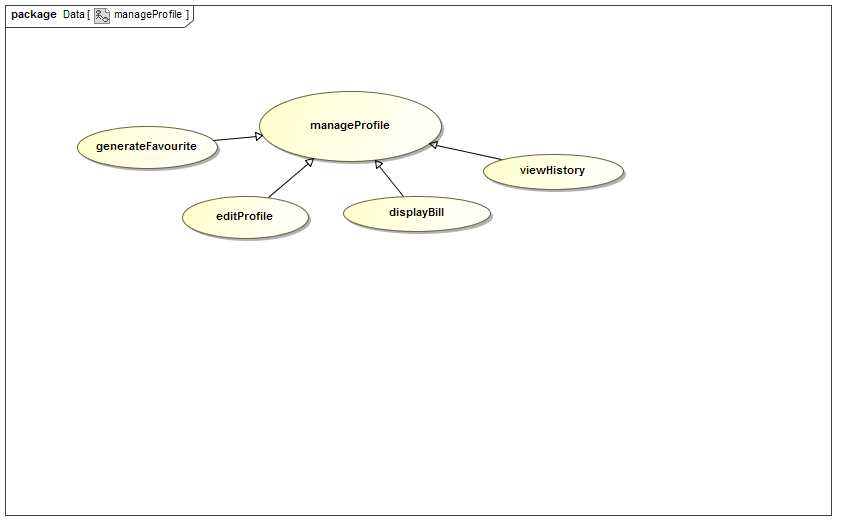
\includegraphics[width=1.0\textwidth]{images/manageProfile.png}
    \caption{The use case diagram for managing profile} 
\end{figure}

\subsubsection{generateFavourite}
The service contract and activity diagram for generateFavourite follow. generateFavourite falls under the use case for Manage Profile (refer to page 11 to view this use case diagram). The user will be able to view their most popular purchases and these will be based on the most recurring item in the user's account history.
\begin{figure}[H]
  \centering
    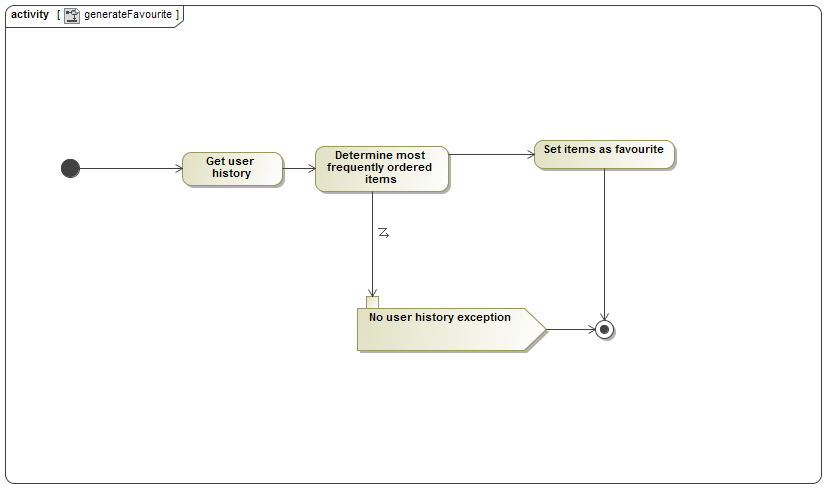
\includegraphics[width=1.0\textwidth]{images/generateFavourite.png}
    \caption{The activity diagram for generating favourites} 
\end{figure}

\begin{figure}[H]
	\centering
	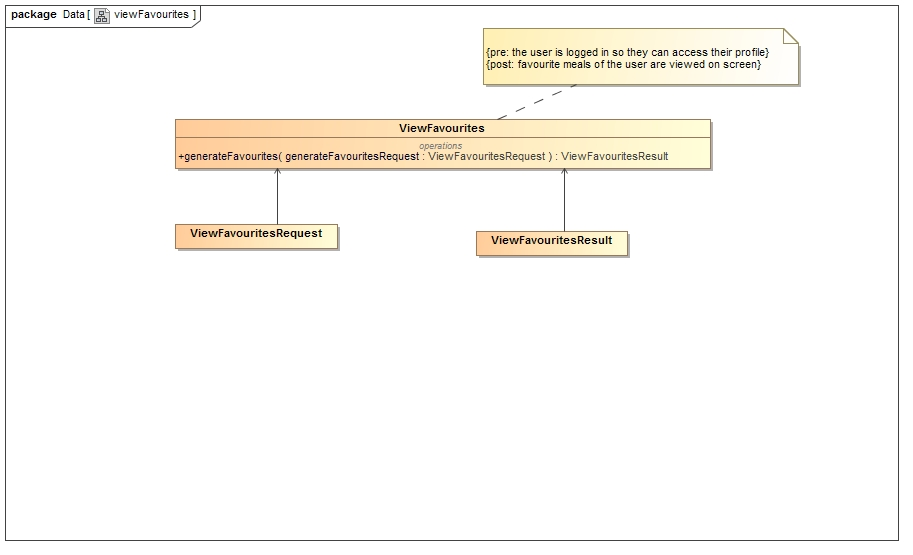
\includegraphics[width=1.0\textwidth]{images/viewFavouritesSC.jpg}
	\caption{The service contract for generating favourites}
\end{figure}

\subsection{editProfile}
Edit profile includes the user changing his/her password and email address as well as changing his/her spending limit. Hence, the following use cases, changePassword, changeEmail and setLimit, are used in the following use case diagram. To view where this use case fits into the system, refer to figure .... 

\begin{figure}[H]
  \centering
    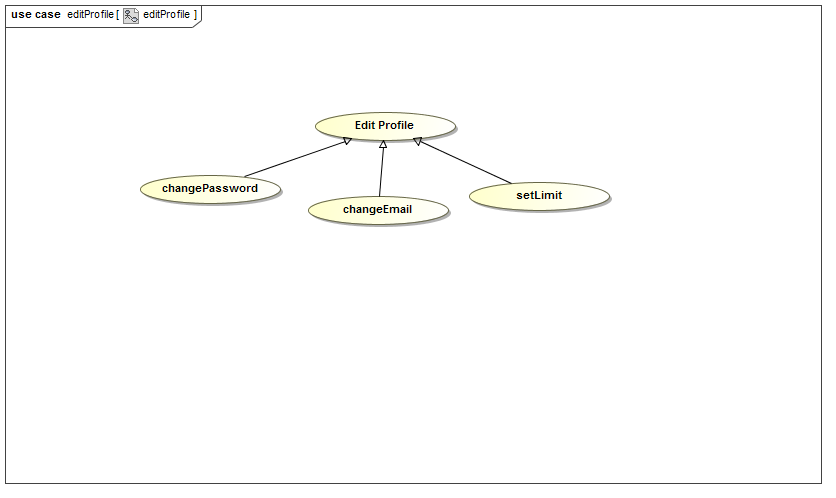
\includegraphics[width=1.0\textwidth]{images/editProfile.png}
    \caption{The use case diagram for editing profile} 
\end{figure}


\subsubsection{changePassword}
The service contract and activity diagram for changePassword follow. changePassword falls under the use case for Edit Profile (refer to page 13 to view this use case diagram). The user will be able to edit their password.
\begin{figure}[H]
  \centering
    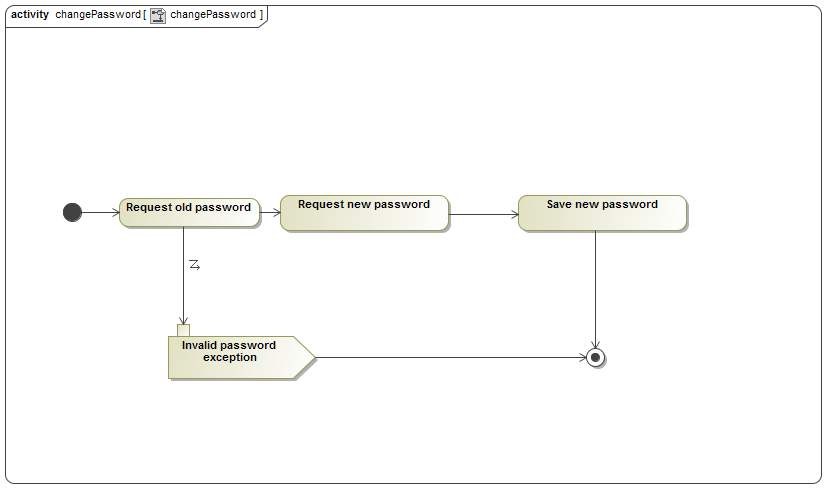
\includegraphics[width=1.0\textwidth]{images/changePassword.png}
    \caption{The activity diagram for changing password } 
\end{figure}
	
\begin{figure}[H]
	\centering
	\includegraphics[width=1.0\textwidth]{images/changePasswordSC.jpg}
	\caption{The service contract for changing password}
\end{figure}

\subsubsection{changeEmail}
The service contract and activity diagram for changeEmail follow. changeEmail falls under the use case for Edit Profile (refer to page 13 to view this use case diagram). The user will be able to edit their email address.
\begin{figure}[H]
  \centering
    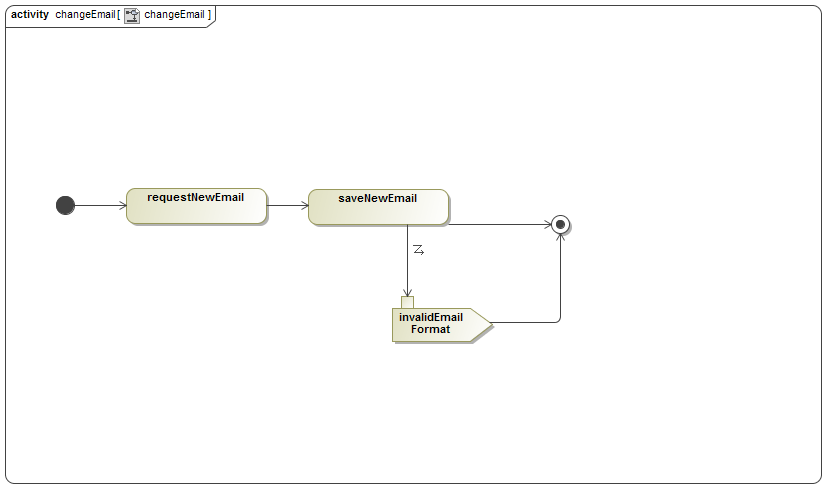
\includegraphics[width=1.0\textwidth]{images/changeEmail.png} 
    \caption{The activity diagram for changing email address}
\end{figure}
	
\begin{figure}[H]
	\centering
	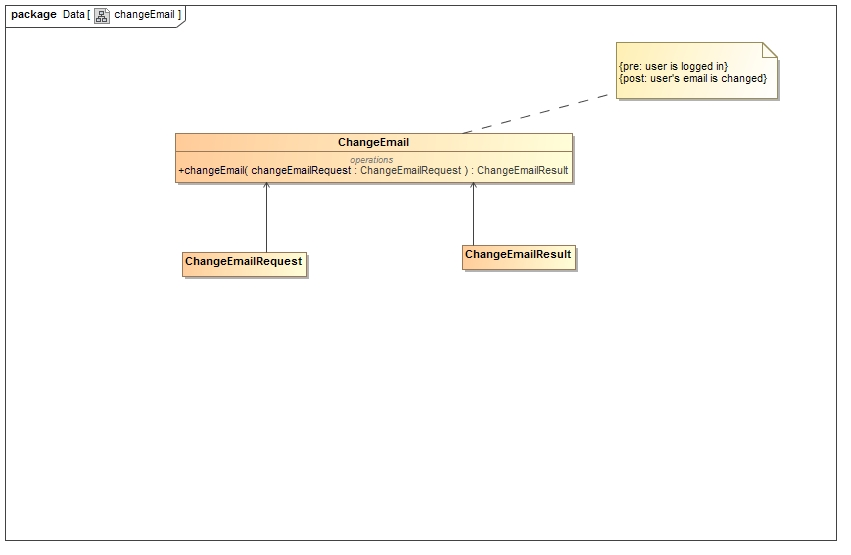
\includegraphics[width=1.0\textwidth]{images/changeEmailSC.jpg}
	\caption{The service contract for changing email address}
\end{figure}

\subsubsection{changeLimit}
The service contract and activity diagram for changeLimit follow. changeLimit falls under the use case for Edit Profile (refer to page 13 to view this use case diagram). The user will be able to change their personal spending limit on their profile, however, this must not exeed the system's limit.
\begin{figure}[H]
  \centering
    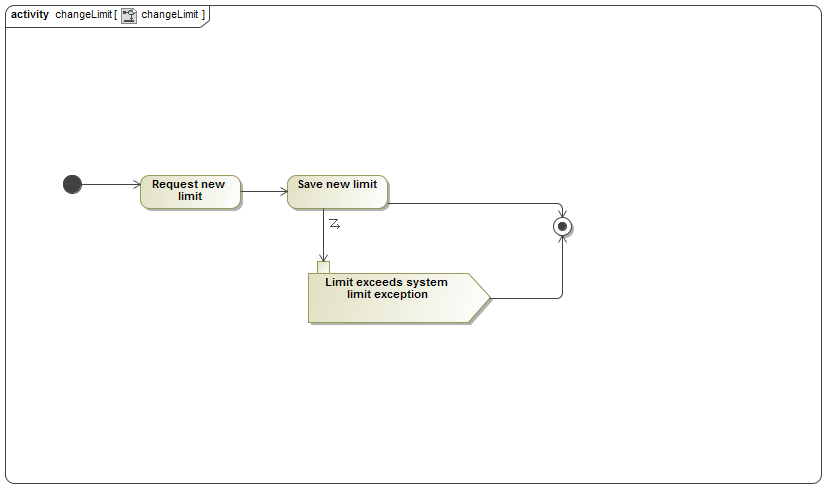
\includegraphics[width=1.0\textwidth]{images/changeLimit.png}
    \caption{The activity diagram for setting limit} 
\end{figure}

\begin{figure}[H]
	\centering
	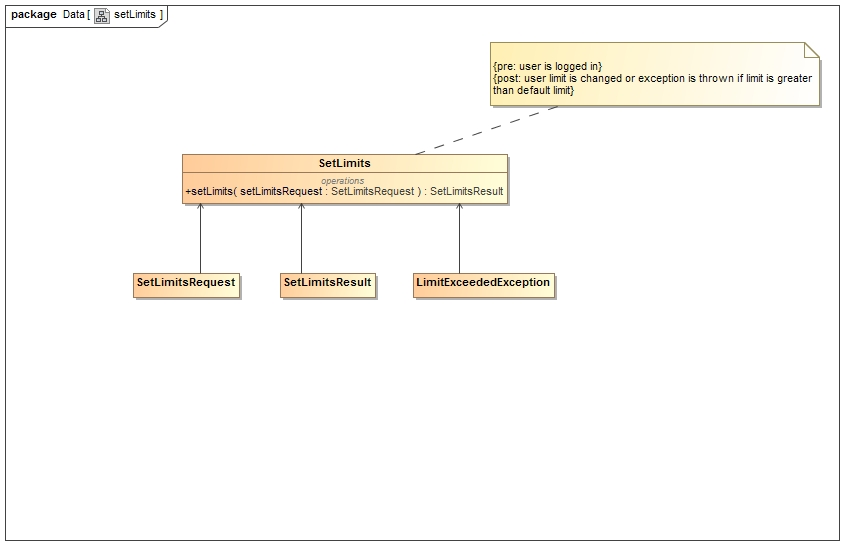
\includegraphics[width=1.0\textwidth]{images/setLimitsSC.jpg}
	\caption{The service contract for setting limit}
\end{figure}
 
\section{Comment}
Due to the fact that an agile approach was followed, the main two modules of the system were explored in this document. As time progresses, the rest of the diagrams will be added and the existing ones will be subject to change.







\end{document}

